\documentclass{article}

\usepackage{aligned-overset}
\usepackage{amsmath}
\usepackage{amssymb}
\usepackage{bbm}
\usepackage[shortlabels]{enumitem}
\usepackage{genealogytree}
\usepackage{hyperref}
\usepackage[utf8]{inputenc}
\usepackage{interval}
\intervalconfig{
  soft open fences
}

\usepackage{mathtools}
\usepackage{physics}
\usepackage{tikz}
\usetikzlibrary{patterns}
\usetikzlibrary{positioning}
\usetikzlibrary{shapes.geometric}
\usepackage{xcolor}
\definecolor{light-gray}{gray}{.9}

\author{Karsten Lehmann}
\date{03.11.2020}
\title{Übung Lineare Algebra - Grundlegende Konzepte}

\begin{document}


\maketitle
\newpage

\subsection*{Übung 1}
\begin{enumerate}
\item Für alle $a \in A \colon a \in B$ kann man auch schreiben als:
  \begin{enumerate}
  \item $A \cap B$
  \item $A = B$
  \item $A \subseteq B$
  \end{enumerate}
  \[
    \forall a \in A \colon a \in B \colon A \subseteq B
  \]
\item Welche der folgenden Terme ergibt eine leere Menge?
  \begin{enumerate}
  \item $A \cup B$
  \item $A \cap B$
  \item $A \setminus A$
  \end{enumerate}
\end{enumerate}

\subsection*{Übung 2}

Seien $A,B,C$ Mengen. Zeigen Sie

\begin{enumerate}
\item
  \[
    A \cap (B \cup C) = \color{blue} (A \cap B) \color{black} \cup \color{red} (A \cap C) 
  \]
  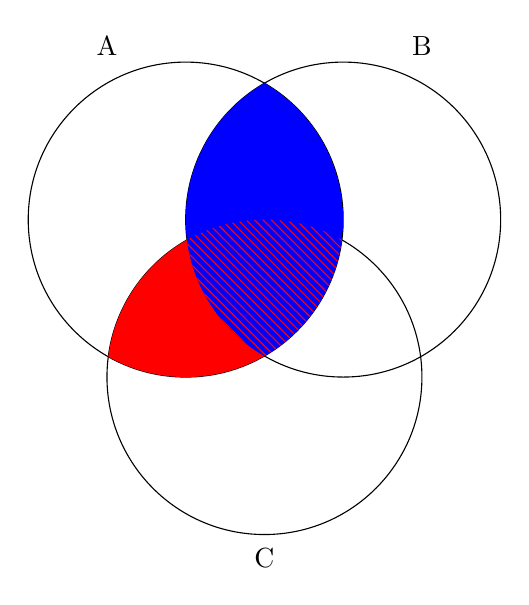
\begin{tikzpicture}    
    \def\circleA{(0,0) circle (2cm)}
    \def\circleB{(2,0) circle (2cm)}
    \def\circleC{(1,-2) circle (2cm)}

    \draw \circleA node[xshift=-1cm, yshift=2.2cm] {A};
    \draw \circleB node[xshift=1cm, yshift=2.2cm] {B};
    \draw \circleC node[yshift=-2.3cm] {C};

    %% Durchschnitt von A und C rot füllen
    \begin{scope}
      \clip \circleA;
      \clip \circleC;
      \fill[red] \circleA; 
    \end{scope}

    %% Durchschnitt von A und B blau füllen
    \begin{scope}
      \clip \circleA;
      \clip \circleB;
      \fill[blue] \circleA; 
    \end{scope}
    
    
    \begin{scope}
      \clip \circleB;
      \clip \circleC;
      \fill[preaction={fill=blue}, pattern color=red, pattern=north west lines] \circleA; 
    \end{scope}

  \end{tikzpicture}
\item
  \begin{align*}
    & A \cup (B \cap C) = (A \cup B) \cap (A \cup C)  \\
    x &\in (A  \cup B) \cap (A \cup C) \\
    &\iff x \in (A \cup B) \text{ und } x \in (A  \cup C) \\
    &\iff x \in A \text{ oder } x \in B \text{ und } x \in A \text{ oder } x \in C \\
    &\iff x \in A \text{ oder } x \in B \text{ und } x \in C \\
    &\iff x \in A \cup (B \cap C) \\
  \end{align*}
\end{enumerate}

\subsection*{Übung 3}

Seien $A, B$ Teilmengen einer Menge $X$. Zeigen Sie die Äquivalenz folgender Aussagen:

\begin{enumerate}
\item $A \cap B = \emptyset$
\item $A \subseteq X \setminus B$
\item $B \subseteq X \setminus A$
\end{enumerate}

\[
  X \setminus B \coloneqq \{ x \in X | x \notin B\}
\]

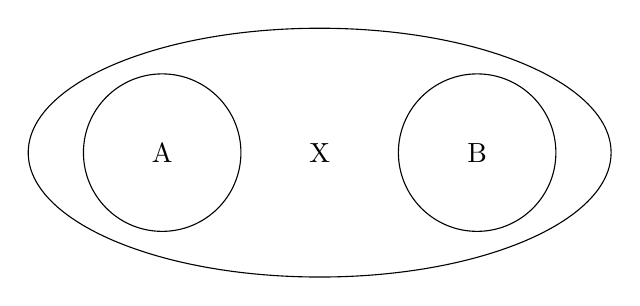
\begin{tikzpicture}
  \node[draw, ellipse, text height = 2cm, text width = 5cm] at (0,0) {};
  \node at (0,0) {X};
  \node[draw, circle, minimum size=2cm] at (-2,0) {A};
  \node[draw, circle, minimum size=2cm] at (2,0) {B};
\end{tikzpicture}

\subsection*{Übung 4}

Sei $M$ eine Menge und seien $A \subseteq M, B \subseteq M$. Wir bezeichnen mit $A^C$ das Komplement von $A$.
Finden Sie eine Menge $X \subseteq M$, die folgende Gleichung erfüllt:

\begin{align*}
  &(X \cup A)^C \cup (X \cup A^C)^C = B \\
  &m \in (X \cup A)^C \text{ oder } m \in (X \cup A^C)^C \\
  &\iff m \in M \setminus (X \cup A) \text{ oder } m \in M \setminus (X \cup A^C) \\
  &\iff m \in M \text{ und } m \notin (X \cup A) \text{ oder } m \in M \text{ und } m \notin (X \cup A^C) \\
  &\iff m \notin X \text{ oder } m \notin A \text{ oder } m \notin X \text{ oder } m \notin A^C \\
  &m \notin X \iff m \in B \\
  &\Rightarrow X = M \setminus B \\
\end{align*}

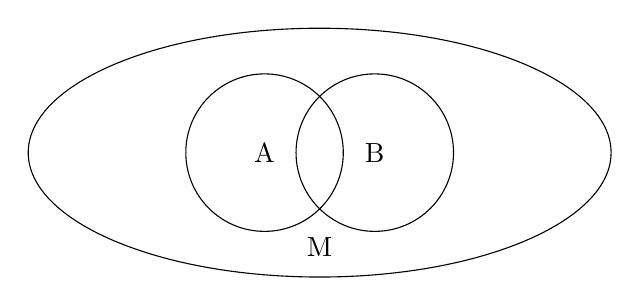
\begin{tikzpicture}
  \node[draw, ellipse, text height = 2cm, text width = 5cm] at (0,0) {};
  \node at (0,-1.2) {M};
  \node[draw, circle, minimum size=2cm] at (-.7,0) {A};
  \node[draw, circle, minimum size=2cm] at (.7,0) {B};
\end{tikzpicture}

\subsection*{Übung 6}

Sei $f \colon X \to Y$ eine Funktion und $A, B \subseteq X, C, D \subseteq Y$. Zeigen Sie die folgenden Aussagen

\begin{enumerate}
\item $f(A \cap B) \subseteq f(A) \cap f(B)$
\item $f(A \cup B) = f(A) \cup f(B)$
\item $X \setminus A \supseteq f(X) \setminus f(A)$
\item $f^{-1}(f(A)) \supseteq A$
\item $f^{-1}(C \cap D) = f^{-1}(C) \cap f^{-1}(D)$
\item $f^{-1}(C \cup D) = f^{-1}(C) \cup f^{-1}(D)$
\item $f^{-1}(Y \setminus C) = X \setminus f^{-1}(C)$
\item $f(f^{-1}(C)) \subseteq $
\end{enumerate}

\newpage

\section*{Präsenzübung 5}

\subsection*{Übung 1}

\begin{enumerate}[(i)]
\item
  Sei $\{ v_1, \ldots, v_n \}$ linear unabhängig.
  $\{ v_{k_1}, \ldots, v_{k_r}\}$ mit $k \in \{ 1, \ldots, r \}$, $r \leq n$
  angenommen $v_{k_1}, \ldots, v_{k_r}$ mit $\lambda_1 \cdot v_{k_1} + \ldots + \lambda_r \cdot v_{k_r} = 0$
  dann erweitere mit $\lambda_{r+1}, \ldots, \lambda_0 = 0$ und erhalte
  $\lambda_1 \cdot v_{k_1} + \ldots + \lambda_r \cdot v_{k_r} + \lambda_{r+1} \cdot v_{k_{r+1}} + \ldots + \lambda_n \cdot v_{k_n} = 0$

\item
  $\{ w_1, \ldots, w_n\}$ eine Menge von Vektoren und $w_{k_1}, \ldots, w_{k_r}$ eine linear abhängige Teilmenge, dann
  $w_1, \ldots, w_n$ linear abhängig.

  Da $\{ w_1, \ldots, w_n\}$ linear abhängig, existieren $\lambda_1, \ldots, \lambda_r$ mit
  $\lambda_1 w_{k_1} + \ldots + \lambda_r w_{k_r} = 0$
  erweitere nun mit $\lambda_{r+1} = \ldots = \lambda_n = 0$
  \[
    \lambda_1 w_{k_1} + \ldots + \lambda_r w_{k_r} = 0 + \lambda_{r+1} w_{k_{r+1}} + \ldots + \lambda_n w_{k_n} = 0 + 0 = 0
  \]

  $\Rightarrow$ damit haben wir nicht triviale Linearkombinationen von $w_1, \ldots, w_n$ gleich $0$, also $w_1, \ldots, w_n$
  linear abhängig.
\end{enumerate}

\subsection*{Übung 2}

Untersuchen Sie folgende Vektoren auf lineare Unabhängigkeit (über $\mathbb{Q}$ und $\mathbb{R}$)


\begin{enumerate}[(i)]
\item
  $v_1 = \begin{pmatrix}1\\2\end{pmatrix}$ und $v_2 = \begin{pmatrix}-1\\1\end{pmatrix}$.
  Zwei Vektoren sind linear Abhängig, genau dann wenn einer der beiden ein Vielfaches des
  anderen ist, also $v_1 = \lambda \cdot v_2$.
  In diesem Fall sind die beiden Vektoren linear unabhängig.

\item
  $v_1 = \begin{pmatrix}1\\2\end{pmatrix}$ und $v_2 = \begin{pmatrix}\sqrt{3}\\\sqrt{12}\end{pmatrix}$.
  \[
    \sqrt{3} \cdot \begin{pmatrix}1\\2\end{pmatrix} = \begin{pmatrix}\sqrt{3}\\2 \cdot \sqrt{3}\end{pmatrix} = \begin{pmatrix}\sqrt{3}\\\sqrt{12}\end{pmatrix} 
  \]
  Also sind $v1$ und $v2$ in $\mathbb{R}$ linear abhängig. In $\mathbb{Q}$ sind die beiden Wurzeln allerdings nicht erhalten.

\item
  $v_1 = \begin{pmatrix}1\\0\\0\end{pmatrix}$;
  $v_2 = \begin{pmatrix}1\\1\\0\end{pmatrix}$;
  $v_3 = \begin{pmatrix}1\\1\\1\end{pmatrix}$

  \[
    \left(
    \begin{array}{ccc|c}
      1 & 1 & 1 & 0 \\
      0 & 1 & 1 & 0 \\
      0 & 0 & 1 & 0 \\
    \end{array}
    \right)
    \rightsquigarrow
    \left(
    \begin{array}{ccc|c}
      1 & 0 & 0 & 0 \\
      0 & 1 & 0 & 0 \\
      0 & 0 & 1 & 0 \\
    \end{array}
    \right)
  \]
  
  $\rightsquigarrow$ damit ist die einzige Lösung trivial: $\lambda_1 = 0 = \lambda_2 = \lambda_3$ und
  $v_1, v_2, v_3$ damit linear unabhängig.
  
\end{enumerate}

\subsection*{Übung 4}

\begin{enumerate}[(i)]
  \setcounter{enumi}{2}
\item $V = \mathbb{R}[t]$, $\mathbb{K} = \mathbb{R}$

  $v_1 = 1 + t - t^2; v_2 = t + t^2; v_3 = 1 + t - t^2 + t^3$

  alle $v_i$ haben höchstens Grad 3.

  \[
    v_1 =
    \begin{pmatrix}
      1 \\
      1 \\
      -1 \\
      0
    \end{pmatrix}
    \begin{array}{cc}
      \leftarrow & t^0 \\
      \leftarrow & t^1 \\
      \leftarrow & t^2 \\
      \leftarrow & t^3 \\
    \end{array}
    v_2 =
    \begin{pmatrix}
      0 \\
      1 \\
      1 \\
      0
    \end{pmatrix}
    v_3 =
    \begin{pmatrix}
      1 \\
      1 \\
      -1 \\
      1
    \end{pmatrix}
  \]

  \[
    \begin{pmatrix}
      1  & 0 & 1  \\
      1  & 1 & 1  \\
      -1 & 1 & -1 \\
      0  & 0 & 1  \\
    \end{pmatrix}
    \rightsquigarrow
    \begin{pmatrix}
      1 & 0 & 1 \\
      0 & 1 & 0 \\
      0 & 1 & 0 \\
      0 & 0 & 1 \\
    \end{pmatrix}
    \rightsquigarrow
    \begin{pmatrix}
      1 & 0 & 1 \\
      0 & 1 & 0 \\
      0 & 0 & 1 \\
      0 & 0 & 0 \\
    \end{pmatrix}
  \]
  $\rightsquigarrow$ also $v_1, v_2, v_3$ linear unabhängig.

\end{enumerate}

\end{document}
